\documentclass[12pt,a4paper,fleqn]{article}
\usepackage{latexsym,graphicx}
\usepackage{iman,extra,isar}
\usepackage{isabelle,isabellesym}
\usepackage{style}
\usepackage{pdfsetup}

\hyphenation{Isabelle}
\hyphenation{Isar}
\isadroptag{theory}

\title{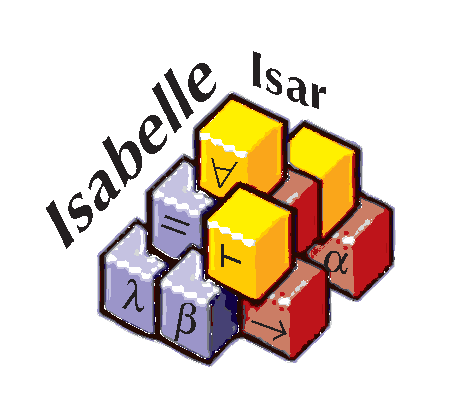
\includegraphics[scale=0.5]{isabelle_isar}
  \\[4ex] The {Isabelle/HOL} type-class hierarchy}
\author{\emph{Florian Haftmann}}

\begin{document}

\maketitle

\begin{abstract}
  \noindent This primer introduces corner stones of the {Isabelle/HOL}
  type-class hierarchy and gives some insights into its internal
  organization.
\end{abstract}

\thispagestyle{empty}\clearpage

\pagenumbering{roman}
\clearfirst

\input{Typeclass_Hierarchy.tex}

\begingroup
\bibliographystyle{plain} \small\raggedright\frenchspacing
\bibliography{manual}
\endgroup

\end{document}
